% This is part of a Thesis Template by Salvador Rodriguez-Gomez.
% This template is inspired in part by several other templates.
% It is distributed under the Creative Commons Attribution-ShareAlike license.
% http://creativecommons.org/licenses/by-sa/3.0/

\chapter{Introduction}
\label{chap_intro}
\epigraph{There were many paths that led up into those mountains, and many passes over them. But most of the passes were infested by evil things and dreadful dangers.}{\textit{The Hobbit, J. R. R. Tolkien}}
\section{Nanoporous materials}
Nanoporous crystals --such as zeolites, metal-organic frameworks (MOFs) or covalent-organic frameworks (COFs), form an interesting family of materials.
Its relevance in the scientific community has been growing in the last decades.
\footnote{Although this growing interest is not restricted to the scientific community.
They have a wide variety of uses, including separation and storage of different compounds.
Most compounds frequently used in the chemical or pharmaceutical industry are naturally found in an impure state and nanoporous materials act as molecular sieves for this indispensable separation.
Synthetic drugs, petroleum industry or purification of metals are examples of the polyvalency of these crystals.}
These nanoporous crystals exhibit a huge variety of structural properties which are characterised by high surface area and pore volume. They possess a wide range of structural topologies with tunable regularity structures and interesting host-guest complexation behaviour \cite{Horike2009}. 
\begin{figure*}[ht]
	\begin{center}
            \centering
	    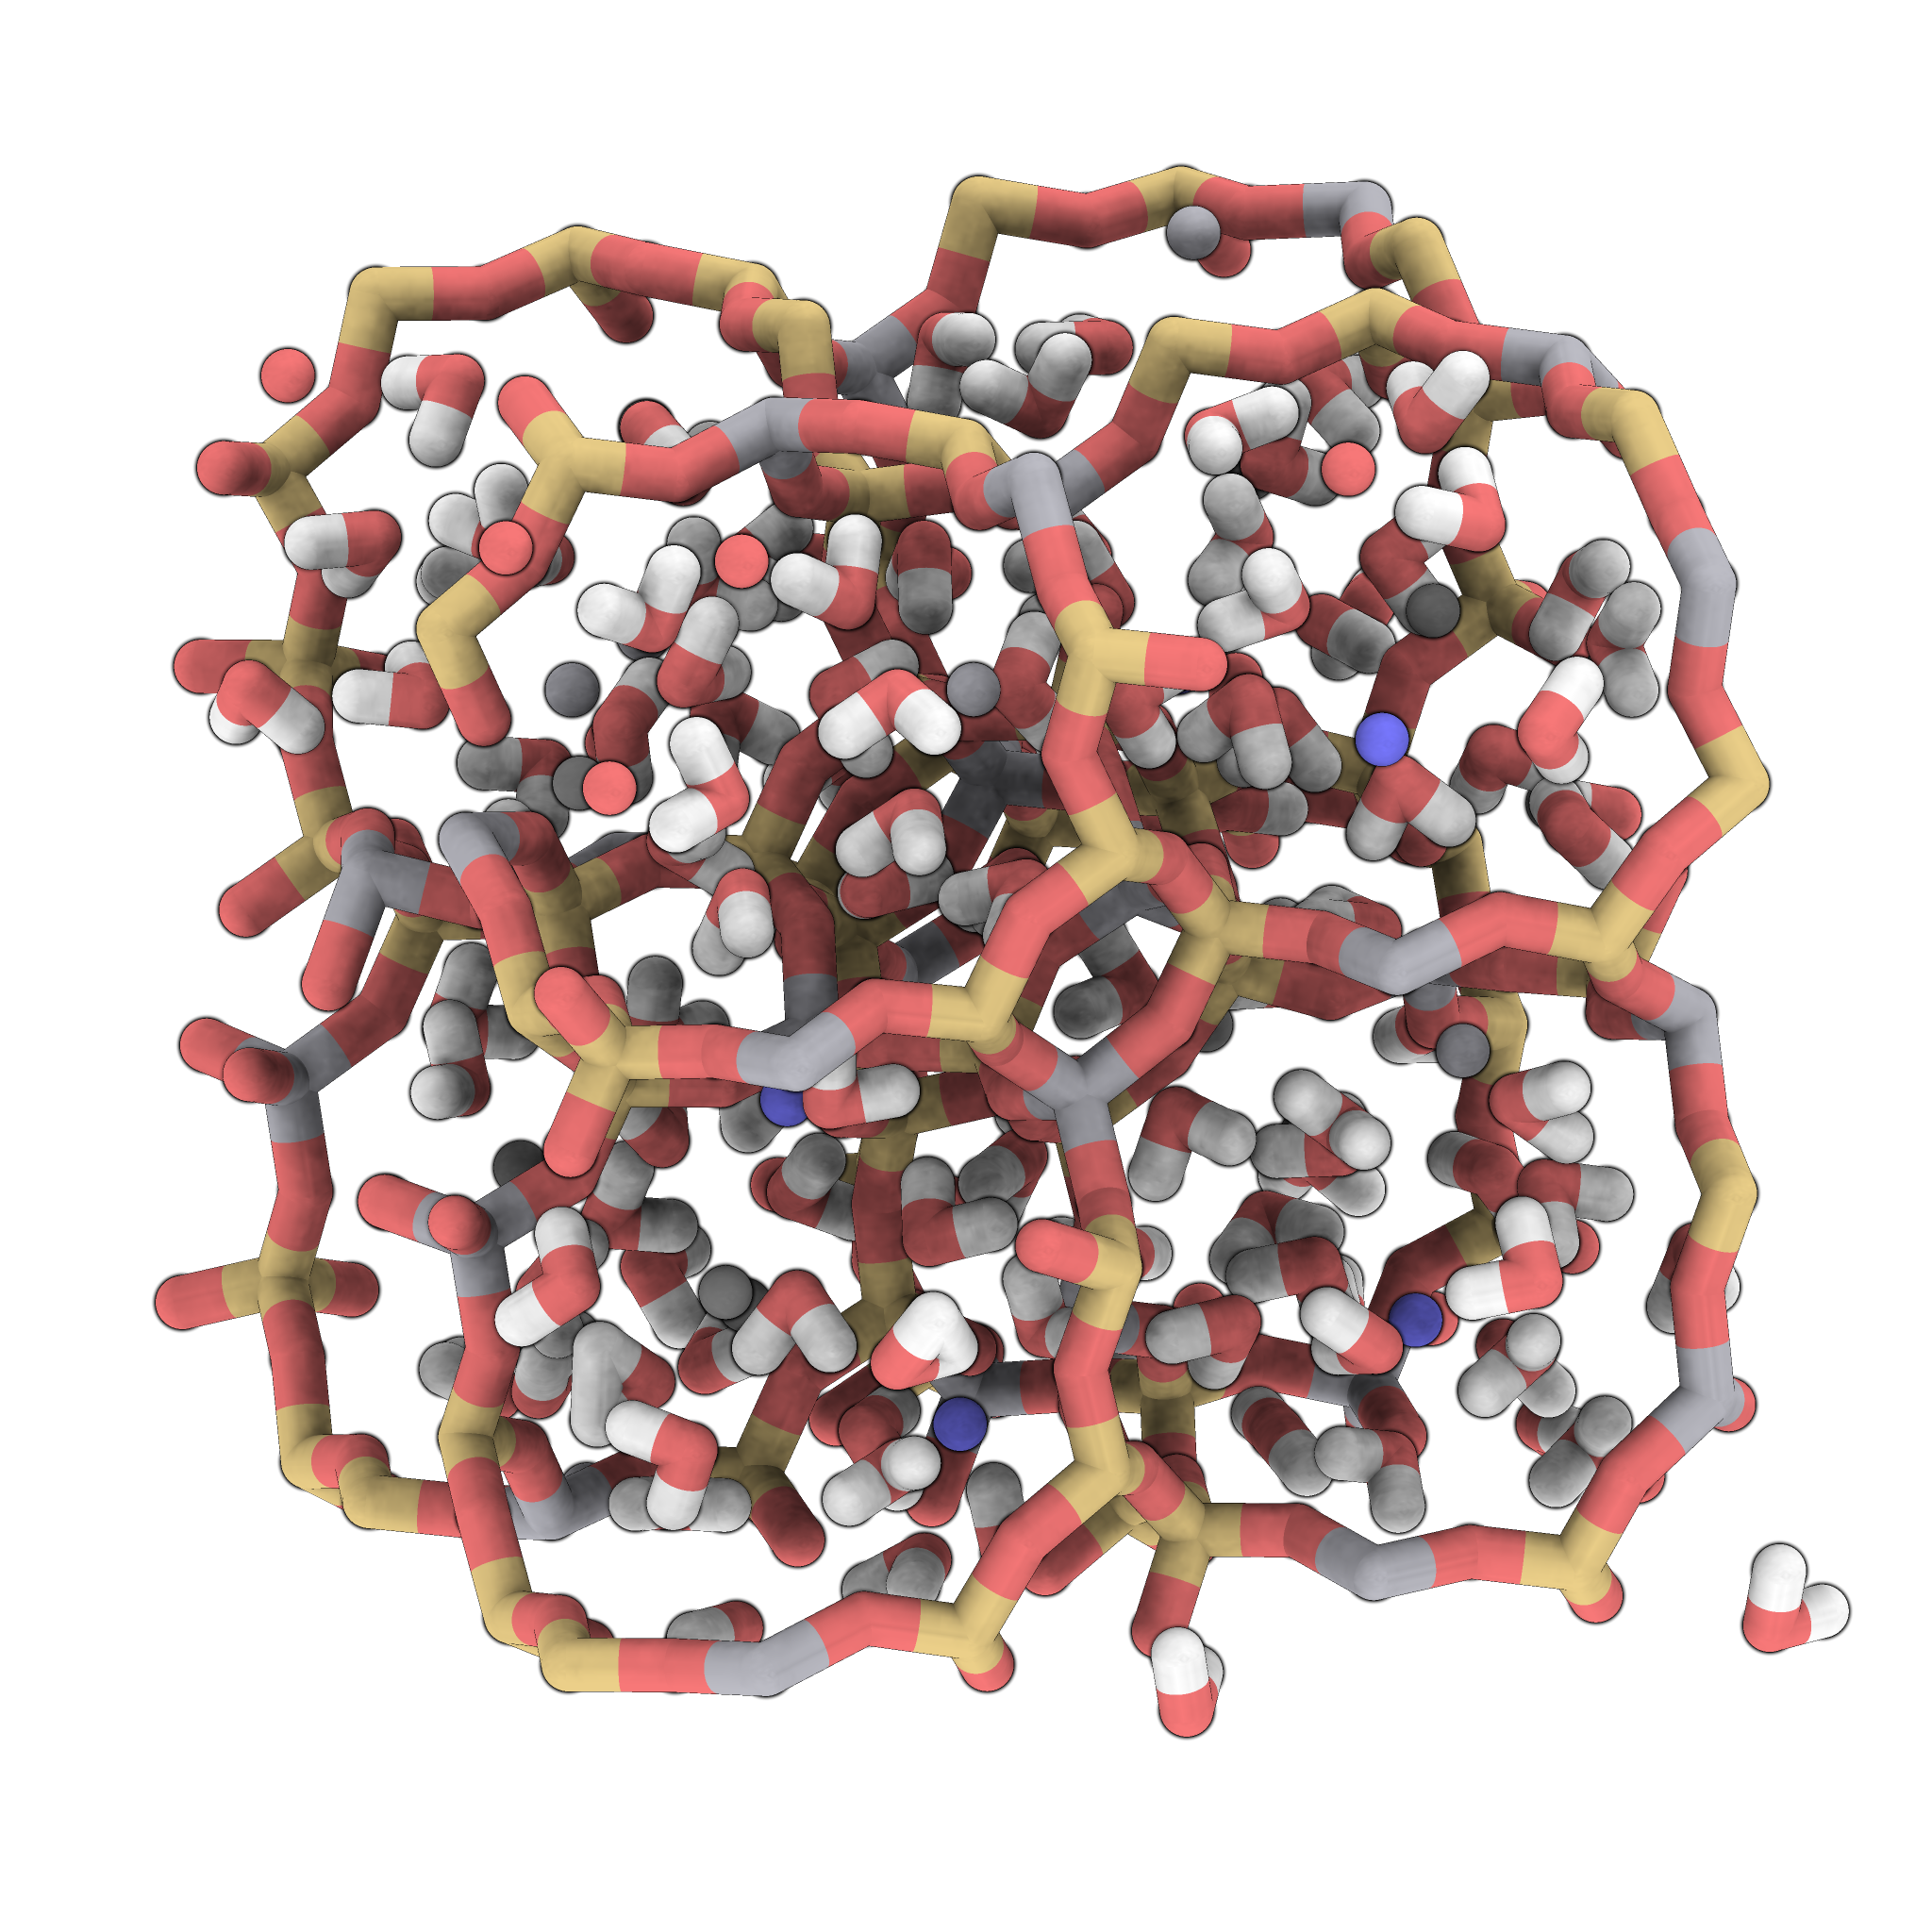
\includegraphics[width=0.45\textwidth]{./introduction/CHA_Na_Ca_water.png}
	    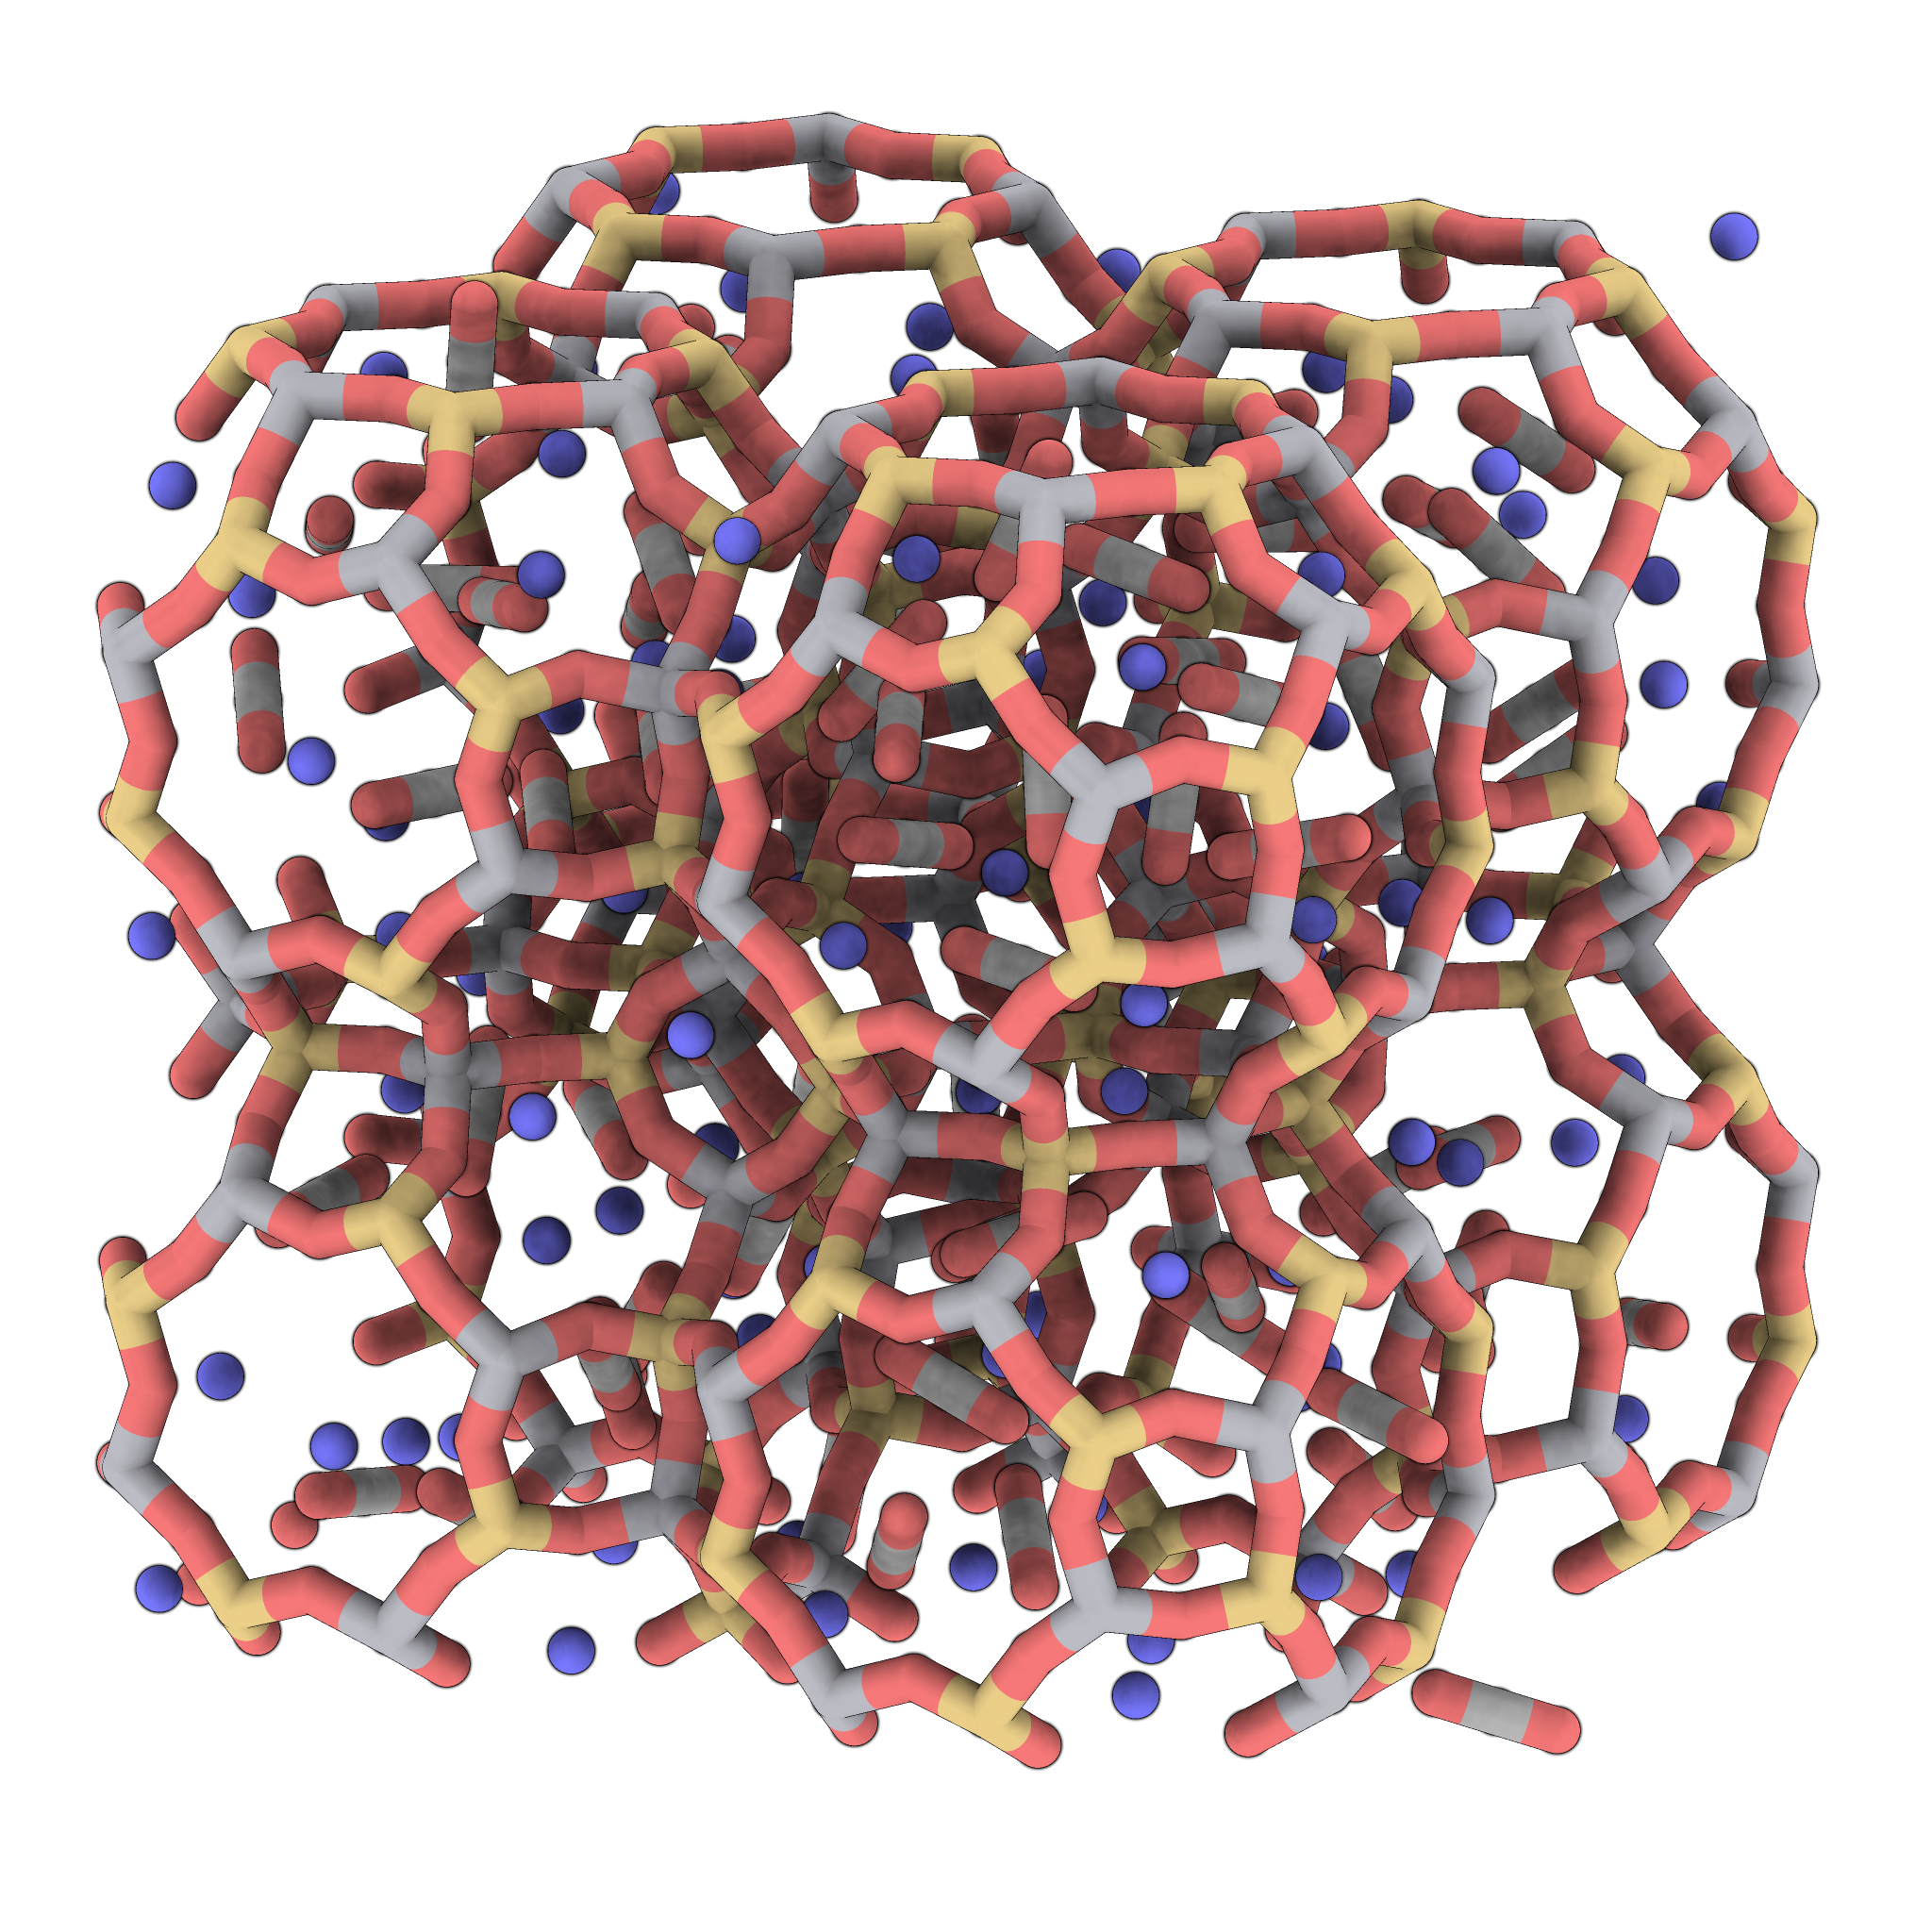
\includegraphics[width=0.45\textwidth]{./introduction/lta5a_co2.png}\\
	    \caption{
            Left: Hydrated CHA-type zeolite or Chabacite with $\text{Si}/\text{Al}=2.5$ with \ce{Na}$^+$ and \ce{Ca}$^{2+}$ cations.
            Right: Adsorption of \ce{CO2} in dehydrated Linde Type A (LTA) with $\nicefrac{\text{Si}}{\text{Al}}=1$ and 96 Na$^+$ per unit cell.
            All snapshots are taken from molecular dynamic simulations at 300 K.}
	    \label{fig:zeolites}
	\end{center}
\end{figure*}

Zeolites were the first porous crystals to be widely studied.
Towards the end of the 1930s zeolitic structures such as analcite, cancrinite, natrolite and sodalite, were reported by \citet{Taylor1930,Pauling453,BRAGG1930} and \citet{Taylor1934}.
Nowadays, more than 230 different zeolite topologies are identified \cite{baerlocher2007atlas} by diffraction techniques.
Zeolites have a three-dimensional framework of TO$_4$ tetrahedra, assembled through oxygen atoms in Secondary Building Units (SBUs) such as cubes (double four--rings or D4R) or octahedra (single eight--ring, S8R), among other configurations.
These units are linked in a way that form a regular 3-dimensional structure (framework), which contains \emph{pores}, \emph{windows} and \emph{channels} of molecular size (circa 3--10~\AA~in diameter).
This porosity is reflected the fact that between 20 and 50\% of the volume of a zeolite structure is empty and, in general, accessible to guest molecules.
The central T atom is usually either silicon or aluminium.
However, in the last decades new materials have been synthesised where the Si$^{4+}$ or Al$^{3+}$ ion are substituted by Ga$^{3+}$, Br$^{3+}$ or Ge$^{4+}$.
Aliovalent substitutions change the overall charge within the framework, but the zeolite must remain neutral.
This negative charge is, then, balanced by an extra-framework cation.
The chemical formula of aluminosilicate zeolite is: Me$^{n+}_{\nicefrac{x}{n}}$[(\ce{AlO2})$_x$(\ce{SiO2})$_{1-x}$]@$w$\ce{H2O}, where Me is the cation (organic or inorganic), $n$ their valence, $x$ the molar fraction of Al atoms and $w$ the number of water molecules in the unit cell of the structure. The Al$^{3+}$/Si$^{4+}$ cation-ordering stability is governed by well-known rules, established by Lowenstein and Dempsey \cite{loewenstein,dempsey_1969}.
They state that no Al-O-Al chains are allowed and the number of Al-O-Si-O-Al chains must be minimised (or, what is equivalent the Al-Al pair distance is maximised).
In some particular cases, however, these rules are broken. 
The presence of divalent cations Me$^{2+}$ allows the Al-O-Si-O-Al chains are stabilised.
As a matter of fact, the heteroatom distribution in zeolite frameworks has been subject of major interest for a long time, with some controversial issues arising, such as the much debated Si$^{4+}$/Ge$^{4+}$ cation distribution.


Extra-framework cations are linked to the oxygen atoms of the framework through relatively weak ionic interactions compared to the stronger covalent bonds of the atoms that form the framework. For this reason, extra-framework cations have a high degree of mobility and can \textit{migrate} from its preferential cation sites to another. We will see that these extra-frameworks cations play a very important role in adsorption properties at zeolites because of their electrostatic nature.

Zeolites normally exhibit high surface area, thermal stability (at high Si/Al ratio at least), ion exchange capacity and, of course, catalytic capacity. 
A notable feature of the high Si/Al ratio zeolites (those that appear in nature, also called natural zeolites) is its hydrophilic character, which is the reason behind the fact that these zeolites are often saturated with water. This hydrophilic character is due to various reasons :
1) relative large ratio of surface area per crystal volume,
2) presence of extra-framework cations,
3) existence of dipoles between crystallographic defects of aliovalent substitutions in tetrahedra.
The two last conditions become weaker as Si/Al ratio increases, which eventually leads to a phase transition from hydrophilic to hydrophobic behaviour for ratios close to  8--10.
As an example of this behaviour we have the silicalite structure (MFI-type pure silica structure or ZSM-5), which has a higher adsorption for paraffin compared to water \cite{Olson1996}.

